\documentclass[10pt]{article}
\usepackage[margin=0.4in]{geometry}
\usepackage{amsmath}
\usepackage{enumitem}
\usepackage{multicol}
\usepackage{tikz}
\usetikzlibrary{shapes.geometric}
\usepackage{soul}

\newcommand{\ds}{\displaystyle}
\newcommand{\on}{\operatorname}


\begin{document}
\newcounter{enumCount}
\pagestyle{empty}
\subsection*{Homework 12 - Math 140 \hfill Name: \underline{\hspace*{2in}}}

\noindent
\textit{Find both partial derivatives of the following functions.}

\begin{enumerate}
\item $h(x,y) = x^2 + 2xy + y^2$
\begin{enumerate}
\begin{multicols}{2}
\item $\dfrac{\partial h}{\partial x} =$
\item $\dfrac{\partial h}{\partial y} =$
\end{multicols}
\end{enumerate}
\vfill

%\item $f(x,y) = x^2 e^y$
%\begin{enumerate}
%\begin{multicols}{2}
%\item $\dfrac{\partial f}{\partial x} =$
%\item $\dfrac{\partial f}{\partial y} =$
%\end{multicols}
%\end{enumerate}
%\vfill

\item $g(x,y) = \dfrac{y}{x+y}$
\begin{enumerate}
\begin{multicols}{2}
\item $\dfrac{\partial g}{\partial x} =$
\item $\dfrac{\partial g}{\partial y} =$
\end{multicols}
\end{enumerate}
\vfill

\item $z = (x^2 + y)^{1/2}$
\begin{enumerate}
\begin{multicols}{2}
\item $\dfrac{\partial z}{\partial x} =$
\item $\dfrac{\partial z}{\partial y} =$
\end{multicols}
\end{enumerate}
\vfill


\item Several level curves for the function $f(x,y) = x^2 - y^2$ are shown below.  Find the partial derivatives at the point $(1,1)$ and draw an arrow starting at the point $(1,1)$ that shows the direction of steepest ascent.

\begin{center}
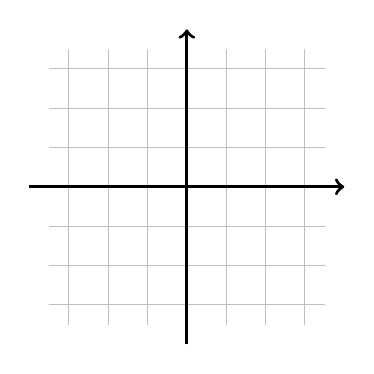
\begin{tikzpicture}[scale=0.5]
  \draw[gray!50] (-3.5,-3.5) grid (3.5,3.5);
  \draw[very thick,blue] plot[raw gnuplot] function{
    f(x,y) = x**2-y**2-0.5;
    set xrange [-4:4];
    set yrange [-4:4];
    set view 0,0;
    set isosample 1000,1000;
    set size square;
    set cont base;
    set cntrparam levels incre 0,0.1,0;
    unset surface;
    splot f(x,y)
  };
  \draw[very thick,blue!80] plot[raw gnuplot] function{
    f(x,y) = x**2-y**2-2;
    set xrange [-4:4];
    set yrange [-4:4];
    set view 0,0;
    set isosample 1000,1000;
    set size square;
    set cont base;
    set cntrparam levels incre 0,0.1,0;
    unset surface;
    splot f(x,y)
  };
  \draw[very thick,blue!60] plot[raw gnuplot] function{
    f(x,y) = x**2-y**2-4.5;
    set xrange [-4:4];
    set yrange [-4:4];
    set view 0,0;
    set isosample 1000,1000;
    set size square;
    set cont base;
    set cntrparam levels incre 0,0.1,0;
    unset surface;
    splot f(x,y)
  };
  \draw[very thick,blue!40] plot[raw gnuplot] function{
    f(x,y) = x**2-y**2-8;
    set xrange [-4:4];
    set yrange [-4:4];
    set view 0,0;
    set isosample 1000,1000;
    set size square;
    set cont base;
    set cntrparam levels incre 0,0.1,0;
    unset surface;
    splot f(x,y)
  };
  \draw[very thick,->] (-4,0) -- (4,0);
  \draw[very thick,->] (0,-4) -- (0,4);
\end{tikzpicture}
\end{center}
\vfill


\item Several level curves for the function $f(x,y) = x^2 + 4y^2$ are shown below.  Find the partial derivatives at the point $(-2,1)$ and draw an arrow starting at the point $(-2,1)$ that shows the direction of steepest ascent.

\begin{center}
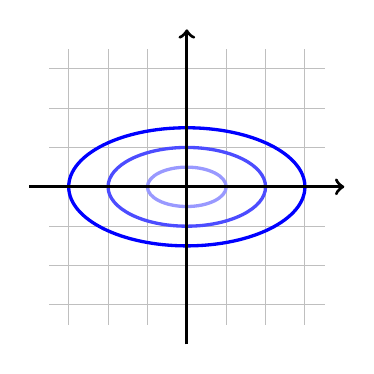
\begin{tikzpicture}[scale=0.5]
  \draw[gray!50] (-3.5,-3.5) grid (3.5,3.5);
  \draw[very thick, blue!40,yscale=0.5] (0,0) circle (1);
  \draw[very thick, blue!70,yscale=0.5] (0,0) circle (2);
  \draw[very thick, blue,yscale=0.5] (0,0) circle (3);
  \draw[very thick,->] (-4,0) -- (4,0);
  \draw[very thick,->] (0,-4) -- (0,4);
\end{tikzpicture}
\end{center}


\newpage
%\item The graph below shows several level curves of the function $f(x,y) = x^2+2x-6y$, and also shows a constraint curve $ y= \frac{6}{x}$.  Without doing any math, estimate the coordinates of the point on the constraint curve where $f(x,y)$ is maximized.  Draw a large dot at that point.  
%
%\begin{center}
%\begin{tikzpicture}[scale=0.5]
%  \draw[gray!50] (-4.5,-5.5) grid (6.5,5.5);
%  %\draw[very thick, blue!40] (0,0) circle (1);
%  %\draw[very thick, blue!55] (0,0) circle (2);
%  %\draw[very thick, blue!70] (0,0) circle (3);
%  %\draw[very thick, blue!85] (0,0) circle (4);
%  %\draw[very thick, blue] (0,0) circle (5);
%  \draw[very thick,color=blue] plot[domain=-3.25:5.25,samples=400] function {(2*x-x**2)/6-2.5};
%  \draw[very thick,color=blue!80] plot[domain=-4.25:6.25,samples=400] function {(2*x-x**2)/6};
%  \draw[very thick,color=blue!60] plot[domain=-4.25:6.25,samples=400] function {(2*x-x**2)/6+2.5};
%  \draw[very thick,color=blue!40] plot[domain=-4.25:6.25,samples=400] function {(2*x-x**2)/6+5};
%  \draw[very thick,->] (-5,0) -- (7,0);
%  \draw[very thick,->] (0,-6) -- (0,6);
%  \draw[very thick,color=red] plot[domain=1.05:7,samples=400] function {6/x} node[right] {$\frac{6}{x}$};
%\end{tikzpicture}
%\end{center}
%
%\item Nitric oxide is a gas can be combined with hydrogen to make oxygen and water. The rate of the chemical reaction is $r = kx^2 y$ where $x$ is the concentration of nitric oxide, $y$ is the concentration of hydrogen, and $k$ is a constant. Find the two partial derivatives $r_x$ and $r_y$. 
%\vfill

\item A cupcake shop can produce $Q(x,y) = 100 x^{1/2} y$ dollars worth of cupcakes in a day where $x$ is hours of labor and $y$ is the number of ovens they have running.  Find the two partial derivatives $Q_x$ and $Q_y$ when $x = 16$ and $y = 1$.  Include the units for each.
\vfill


%\item Using the partial derivatives from the previous problem to estimate how much more money the cupcake shop could make if they purchase a second oven and hire a part-time worker who will work 4 extra hours per day. Use the formula:
%$$\Delta Q = \frac{\partial Q}{\partial x} \Delta x + \frac{\partial Q}{\partial y} \Delta y.$$
%\vfill


%\item A 10-year bond lets you invest $x$ dollars at an interest rate of $r$.  The value of the bond when it matures will be $B(x,r) = x(1+r)^{10}$.  Find the partial derivatives of $B$ with respect to $x$ and $r$.  Then use a calculator to find the values of the two partial derivatives when $x = 100$ and $r = 0.04$.  
%\vfill

\item A factory employs two types of workers.  They have $x$ skilled workers and $y$ unskilled workers.  The total output of the factory is $Q(x,y) = 10x^{0.6} y^{0.4}$.  Find the marginal productivity of skilled and of unskilled workers when $x=50$ and $y=50$.  The marginal productivity of an input is the partial derivative of output with respect to that input.  
\vfill

\item Find the $(x,y)$-coordinates of the critical point of $f(x,y) = x^2 + 2y^2 - xy + 14x$.  
\vfill

\item Use the second derivative test to determine if the critical point from the last problem is a local max, local min, or saddle point.  
\vfill

\item Find the $(x,y)$-coordinates of all critical points of $z = x^2 - 4x + 2y^3 - 9y^2$. 
\vfill

\item Use the second derivative test to classify each critical point from the last problem as a local max, local min, or saddle point.  
\vfill

\end{enumerate}


\end{document}
